\documentclass[crop=false, class=book]{standalone}


\usepackage{graphicx}
\usepackage[italian]{varioref}
\usepackage{copyrightbox}

\begin{document}
		
	\chapter{Depth understanding}
	
		\section{Depth API}
	
			ARCore Depth API aggiunge un livello di realismo attraverso l'uso di algoritmi che generano immagini o mappe di profondità. Questi algoritmi sono in grado di ottenere stime di profondità fino a 65 metri. Un'immagine di profondità (figura \vref{fig: depth-map}) offre una visualizzazione 3D del mondo reale, ogni pixel è associato alla distanza dalla scena e attraverso l'uso di colori differenti è possibile riconoscere quali aree dello spazio sono più vicine al dispositivo. La profondità viene acquisita con piccoli spostamenti dai quali si ottengono misure più efficienti (fino a 5 metri). Per ciascun frame può essere recuperata l'immagine di profondità corrispondente dopo che l'utente abbia iniziato a muoversi con il dispositivo. Depth API richiede una grande potenza di elaborazione ed è supportata solo da alcuni dispositivi; è necessario controllare se il dispositivo è compatibile e nel caso lo fosse attivare la profondità manualmente nella configurazione della sessione ARCore.\\
		 	Le principale funzionalità offerte da depth API sono tre:
		\begin{itemize}
			\item[•] \textbf{Copertura dei contenuti}: permette di posizionare accuratamente dei contenuti virtuali di fronte o dietro degli oggetti reali.
			\item[•] \textbf{Immersione}: permette di decorare una scena con oggetti virtuali che interagiscono tra di loro.
			\item[•] \textbf{Interazione}: i contenuti virtuali sono in grado di interagire con il mondo reale attraverso cambiamenti fisici e collisioni.
		\end{itemize}
		
			\begin{figure}
				\centering
				\copyrightbox[0.5]{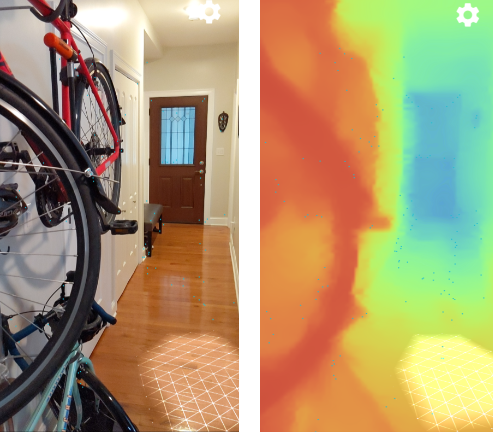
\includegraphics[width=0.5\textwidth]{./resources/images/depthAPI/DepthMap.png}}%
				{Fonte: \url{https://developers.google.com/ar/develop/depth}}
				\caption{Esempio di mappa di profondità}
				\label{fig: depth-map}
			\end{figure}	
		
		\clearpage
		
		\subsection{Sessione ARCore con depth API}
		
			Prima di iniziare una nuova sessione ARCore è necessario controllare se il dispositivo supporta depth API. A volte questa opzione può essere disattivata oppure non supportata nonostante il dispositivo supporti ARCore. Dopo aver definito la sessione con le opportune configurazioni è possibile controllare se il dispositivo e la fotocamera supportano una determinata modalità di profondità invocando il metodo \textbf{isDepthModeSupported(Config.DepthMode mode)} sull'istanza della sessione. Se la modalità è supportata viene configurata la sessione e sarà possibile sfruttare depth API \cite{google2022depth}. (Codice \vref{lst: check-api-depth})\\
		
			\begin{center}
				\begin{minipage}{0.95\textwidth}
					\begin{lstlisting}[caption={ Controllo supporto depth API}, label={lst: check-api-depth}, language=Kotlin]
				
					val config = session.config

					// Check whether the user's device supports the Depth API.
					val isDepthSupported = session.isDepthModeSupported(Config.DepthMode.AUTOMATIC)
					if (isDepthSupported) {
  						config.depthMode = Config.DepthMode.AUTOMATIC
					}
					session.configure(config)
				
					\end{lstlisting}
			\end{minipage}
		\end{center}
		
		\begin{flushleft}
		Per ottenere l'immagine di profondità relativa al frame corrente viene invocato il metodo \textbf{acquireDepthImage16Bits()}.(Codice \vref{lst: depth-image})\\
		\end{flushleft}
		
		\begin{center}
				\begin{minipage}{0.95\textwidth}
					\begin{lstlisting}[caption={ Estrazione di un'immagine profonda}, label={lst: depth-image}, language=Kotlin]
					val frame = arFragment.arSceneView.frame

					// Retrieve the depth image for te current frame, if available
					try{
						frame.acquireDepthImage16Bits().use{ depthImage ->
							//Use the depth image here
						}
					} catch(e: NotYetAvailableException){
						// This means that depth data is not available yet.
  						// Depth data will not be available if there are no tracked
  						// feature points. This can happen when there is no motion, or when the
  						// camera loses its ability to track objects in the surrounding
  						// environment. 
					}
					
					\end{lstlisting}
			\end{minipage}
		\end{center}
		\clearpage
		\begin{center}
				\begin{minipage}{0.95\textwidth}
					\begin{lstlisting}[caption={ Estrazione di informazioni da un'immagine profonda}, label={lst: inf-depth-img}, language=Kotlin]
					/** Obtain the depth in millimeters for [depthImage] at coordinates ([x], [y]). */
					fun getMillimetersDepth(depthImage: Image, x: Int, y: Int): Int {
					
  						// The depth image has a single plane, which stores depth for each
  						// pixel as 16-bit unsigned integers.
  						val plane = depthImage.planes[0]
  						
  						//The distance between adjacent pixel samples, in bytes
  						val pixelStride= x * plane.pixelStride
  						
  						//The row stride for this color plane, in bytes.
  						val rowStride= y * plane.rowStride
  						
  						val byteIndex = pixelStride + rowStride 
  						
  						//Retrieves this buffer's byte order. 
  						val buffer = plane.buffer.order(ByteOrder.nativeOrder())
  					
  						//Reads two bytes at the given index, composing them into a short value
  						// according to the current byte order.
  						val depthSample = buffer.getShort(byteIndex)
  						
  						return depthSample.toInt()
					}
					
					\end{lstlisting}
			\end{minipage}
		\end{center}
		
		\section{Raw Depth API}
		Le ARCore Raw Depth API forniscono informazioni più precise sulla profondità di alcuni pixel di un'immagine e permettono di rappresentare la geometria della scena generando delle \textbf{immagini di profondità grezze}. A 					queste immagini vengono associate delle \textbf{immagini di affidabilità} che stabiliscono il grado di confidenza di ciascun pixel (associato ad un valore di profondità) \cite{mobilear2021rawdepth}. In particolare, ogni pixel è un 				numero intero senza segno a 8 bit che indica la stima della confidenza con valori compresi tra 0 (più bassa) e 255 (più alta) inclusi. I pixel senza una stima della profondità valida hanno un valore di confidenza pari a 0 e un valore di profondità nullo.
		
		\begin{figure}
				\centering
				\copyrightbox[0.5]{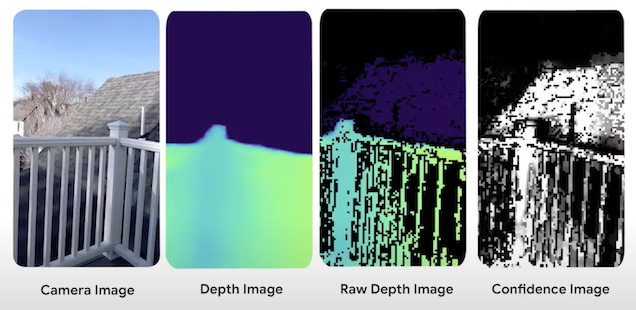
\includegraphics[width=0.8\textwidth]{./resources/images/depthAPI/deptRawAPI.png}}%
				{Fonte: \url{https://stackoverflow.com/questions/59088045/arcore-raw-depth-data-from-rear-android-depth-camera}}
				\caption{Differenze tra immagini in API Raw Depth }
				\label{fig: depth-raw-api}
		\end{figure}
		
		\begin{flushleft}
			L'uso di Raw Depth API è molto utile nei casi in cui c'è il bisogno di avere una maggiore precisione, ad esempio nella \textbf{misurazione} (PHORIA ARConnect App), \textbf{ricostruzione 3d}  (3d Live Scanner App), \textbf{rilevamento delle forme} (Jam3).
			
		\end{flushleft}
		
		\begin{figure}
				\centering
				\copyrightbox[0.5]{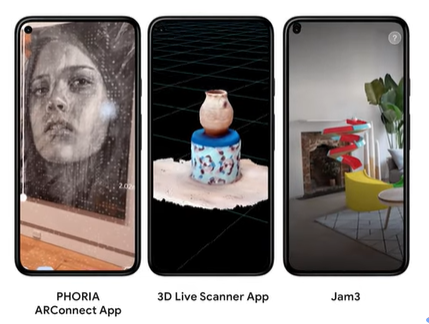
\includegraphics[width=0.6\textwidth]{./resources/images/depthAPI/deptRawAPI2.png}}%
				{Fonte: \url{https://www.youtube.com/watch?v=13WugTMOdSs}}
				\caption{Applicazioni Raw Depth API }
				\label{fig: app-depth-raw-api}
		\end{figure}
		\subsection{Sessione ARCore con Raw depth API}
		
		Inizialmente si deve effettuare il controllo sulla compatibilità del dispositivo come riportato nel codice \vref{lst:check-api-depth }.\\
		Per acquisire un'immagine di confidenza viene invocato il metodo \textbf{acquireRawDepthConfidenceImage()}, dalla quale si può ricavare l'accuratezza di ogni pixel di profondità non elaborato \cite{google2022rawdepth}. (Codice 				riportato \vref{lst: confidence-image})
		
		\begin{center}
				\begin{minipage}{0.95\textwidth}
					\begin{lstlisting}[caption={Estrazione di un'immagine di confidenza}, label={lst: confidence-image}, language=Kotlin]
					 try {
					 
					 	//First of all, retrieve raw depth image
  						// Raw Depth image is in uint16, at GPU aspect ratio, in native orientation.
  						frame.acquireRawDepthImage16Bits().use { rawDepth ->
  						
    						// Confidence image is in uint8, matching the depth image size.
    						frame.acquireRawDepthConfidenceImage().use { rawDepthConfidence ->
    						
      							// Compare timestamps to determine whether depth is is based on new
      							// depth data, or is a reprojection based on device movement.
     							 val thisFrameHasNewDepthData = frame.timestamp == rawDepth.timestamp
     							 
      							if (thisFrameHasNewDepthData) {
      							
        							val depthData = rawDepth.planes[0].buffer
        							val confidenceData = rawDepthConfidence.planes[0].buffer
        							val width = rawDepth.width
        							val height = rawDepth.height
        							someReconstructionPipeline.integrateNewImage(
          							depthData,
          							confidenceData,
         						 	width = width,
          							height = height
        							)
      							}
    						}
  						}
					} catch (e: NotYetAvailableException) {
  						// Depth image is not (yet) available.
					}
					
				\end{lstlisting}
			\end{minipage}
		\end{center}
		
		\section{Depth Hit Test}
		
		Integrando la profondità sono stati ottenuti degli hit test più precisi grazie ai quali è possibile posizionare contenuti virtuali anche su superfici non piane in aree con bassa texture \cite{google2022depth}. (Codice in \vref{lst: Depth Hit Test})\\

		\begin{center}
				\begin{minipage}{0.95\textwidth}
					\begin{lstlisting}[caption={Depth Hit Test}, label={lst: Depth Hit Test}, language=Kotlin]
					 val frame = arFragment.arSceneView.frame
					
					 val hitResultList: List<hitResult> = frame.hitTest(tap)
					
					 for(hit in hitResultList){
						 val trackable: Trackable=hit.trackable
						
						 if(trackable is Plane || trackable is Point || trackable is DepthPoint){
							 val anchor=hit.createAnchor()
							 //Use anchor here
						 }
					}
					
				\end{lstlisting}
			\end{minipage}
		\end{center}
		
		
		\section{Depth Lab}
		
		Depth Lab è una libreria software che incapsula un insieme ristretto di depth API grazie alle quali è possibile recuperare risorse utili per \textbf{rilevamento } della geometria e \textbf{rendering} nell'interazione AR. (Figura 			\vref{fig: depthlab})
		
		\begin{figure}
				\centering
				\copyrightbox[b]{\includegraphics[width=1\textwidth]{./resources/images/depthAPI/depthLab.png}}%
		{Fonte: \url{https://augmentedperception.github.io/depthlab/assets/Du_DepthLab-Real-Time3DInteractionWithDepthMapsForMobileAugmentedReality_UIST2020.pdf}}
				\caption{Panoramica ad alto livello di Depth Lab}
				\label{fig: depthlab}
		\end{figure}
		
		\begin{flushleft}
			Depth Lab è costituito da quattro componenti \cite{ruofeidu2020depthlab}:
		\end{flushleft}
		
		\begin{itemize}
			\item[•] \textbf{ Tracking and Input}: vengono utilizzate immagini di profondità (ottenute da Depth API), posa del dispositivo, altri parametri della fotocamera per stabilire la mappatura del mondo fisico e degli oggetti virtuali nella scena.
			\item[•] \textbf{Data structure}: i valori di profondità associati a ciascun pixel sono memorizzati all'interno di un'immagine prospettica (a bassa risoluzione).\\
			 Esistono 3 strutture dati differenti:
			\begin{itemize}
				\item[-] \emph{array di profondità}: memorizza la profondità in un array 2D di un'immagine orizzontale con numeri interi a 16 bit. E' possibile ricavare il valore della profondità di un qualsiasi punto dello schermo.
				\item[-] \emph{mesh di profondità}: fornisce una ricostruzione 3D in tempo reale dell'ambiente circostante per ciascuna mappa di profondità. In figura (a) in \vref{fig: mesh-depth} è rappresentata un'immagine di profondità che specifica il valore di profondità di ciascun pixel in base al colore (i pixel più luminosi indicano regioni più lontane). Ognuno di questi valori verrà proiettato nel template mesh tassellato generando una mesh di profondità in tempo reale (c) costituita dall'interconnessione di superfici triangolari  
				\item[-] \emph{texture della profondità} è una texture che rappresenta la profondità della scena inquadrata dalla fotocamera.
			\end{itemize}
			\item[•] \textbf{Conversion Utilities and Algorithm }: l'utilizzo di algoritmi di conversione è diverso a seconda della funzionalità che viene offerta. Per gestire la fisica dell'ambiente, ombre, occlusione, mappatura di texture e molto altro sono necessari diversi approcci per l'elaborazione della profondità.
			
			\item[•] \textbf{DepthLab Algorithms}: sulla base delle strutture dati gli algoritmi si dividono in 3 categorie:
				\begin{itemize}
					\item[-] \emph{profondità localizzata}: adatto per calcolare misurazioni fisiche, stimare vettori normali, muovere avatar virtuali in giochi AR (creare dei percorsi per evitare che l'avatar collida con qualche oggetto come nella figura \vref{fig: path-avatar}). Utilizza l'array di profondità per operare su un numero ridotto di punti.
					\item[-] \emph{profondità superficiale}: aggiorna mesh di profondità per gestire collisioni, texture decal ( texture che vengono applicate su una superficie di un oggetto con una specifica proiezione), fisica dell'ambiente, riconoscimento geometrico delle ombre. (Esempi in figura \vref{fig: surfaces-depth})
					\item[-] \emph{profondità densa}: utilizzato sul rendering di effetti sensibili alla profondità, riilluminazione, messa a fuoco, occlusione. (Esempi in figura \vref{fig: dense-depth})
				\end{itemize}
			
		\end{itemize}
					
		\begin{figure}
				\centering
				\copyrightbox[b]{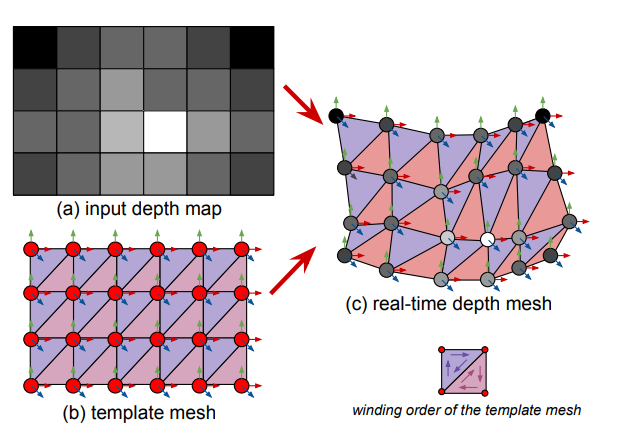
\includegraphics[width=0.6\textwidth]{./resources/images/depthAPI/meshmap.png}}%
				{Fonte: \url{https://augmentedperception.github.io/depthlab/assets/Du_DepthLab-Real-Time3DInteractionWithDepthMapsForMobileAugmentedReality_UIST2020.pdf}}
				\caption{Generazione di una depth mesh }
				\label{fig: mesh-depth}
		\end{figure}
		
		\begin{figure}
				\centering
				\copyrightbox[b]{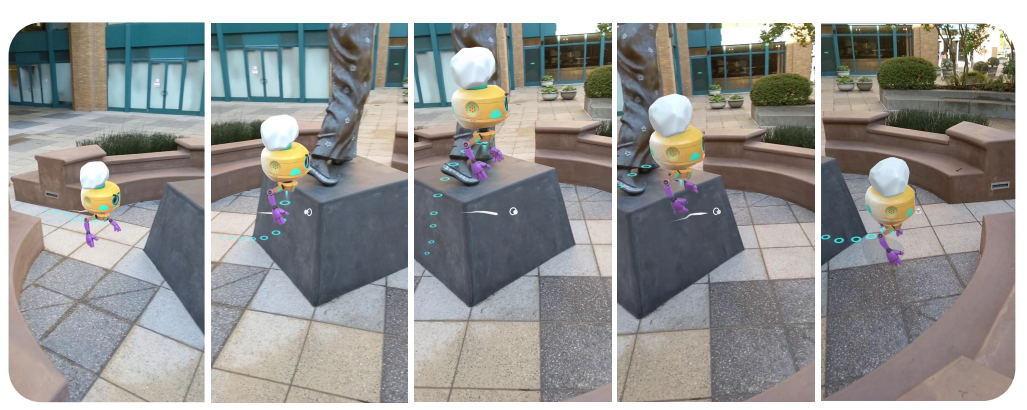
\includegraphics[width=0.8\textwidth]{./resources/images/depthAPI/pathplanning.png}}%
				{Fonte: \url{https://augmentedperception.github.io/depthlab/assets/Du_DepthLab-Real-Time3DInteractionWithDepthMapsForMobileAugmentedReality_UIST2020.pdf}}
				\caption{Pianificazione di un percorso per un avatar virtuale}
				\label{fig: path-avatar}
		\end{figure}
		
		\begin{figure}
				\centering
				\copyrightbox[b]{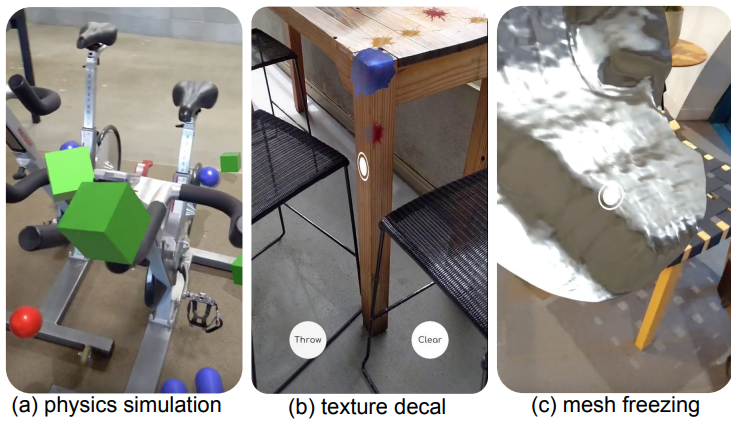
\includegraphics[width=0.7\textwidth]{./resources/images/depthAPI/surfacesdepth.png}}%
				{Fonte: \url{https://augmentedperception.github.io/depthlab/assets/Du_DepthLab-Real-Time3DInteractionWithDepthMapsForMobileAugmentedReality_UIST2020.pdf}}
				\caption{Esempi di profondità superficiale}
				\label{fig: surfaces-depth}
		\end{figure}
		
		\begin{figure}
				\centering
				\copyrightbox[b]{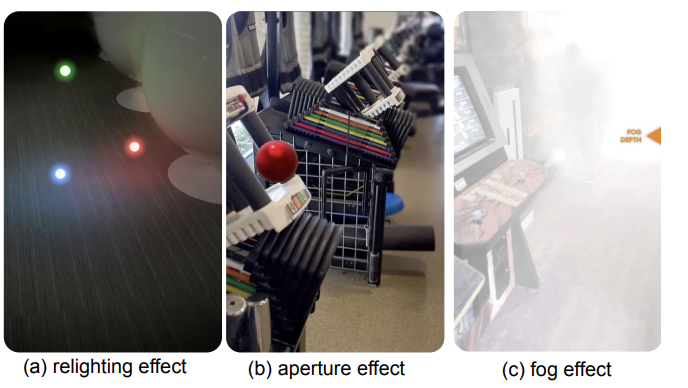
\includegraphics[width=0.7\textwidth]{./resources/images/depthAPI/densedepth.png}}%
				{Fonte: \url{https://augmentedperception.github.io/depthlab/assets/Du_DepthLab-Real-Time3DInteractionWithDepthMapsForMobileAugmentedReality_UIST2020.pdf}}
				\caption{Esempi di profondità densa}
				\label{fig: dense-depth}
		\end{figure}
\end{document}